\section{Modelierung \buch{p.1}}
\subsection{Modellierung eines Embedded Systems}

\begin{itemize}
	\item Modelle werden als Werkzeuge der Dokumentation angesehen. Dadruch 
	wird unter Umständen dasselbe zweimal beschrieben (als Code und als Diagramme)
	
	\item Ziel ist es aus formalen Modellen lauffähige Software erzeugt werden kann. Bei 
	State Machine ist dies durch Statechart der Automaten vollständig möglich.
\end{itemize}

\textbf{Agile Softwareentwicklung}\\
Agile Softwareentwicklung ist der Oberbegriff für den Einsatz von Agilität (flink, beweglich) in der Softwareentwicklung.
\begin{itemize}
	\item Eher offen für Änderungen als starres Festhalten an Plänen
	\item Eher Menschen und Kommunikation als Prozesse und Tools
	\item Eher "darüber miteinander reden" als "gegeneinander schreiben"
	\item Eher Vertrauen als Kontrolliren
	\item Eher "Best Practices" aus Erfahrung als verordnete Vorgaben
	\item Eher Angemessenheit als Extremismus
	\item \textbf{Aber keine Anarchie!}
\end{itemize}

\textbf{Model Driven Development}\\
Bei der modellbasierten Entwicklung kommen in allen Entwicklungsphasen durchgängig Modelle zur Anwendung.\\\\

\begin{multicols}{2}
	\textbf{UML:}
	\begin{itemize}
		\item Aktivitätsdiagramm
		\item Sequenzdiagramm
		\item Zustandsdiagramm
		\item Klassendiagramm
		\item Use Case Diagramm
		\item Verteilungsdiagramme
	\end{itemize}
	\columnbreak
	
	\textbf{Vorgehen bei Modellierung:}
	\begin{enumerate}
		\item Systemgrenze Definieren
		\item Systemprozesse finden
		\item Verteilung festlegen
		\item Systemprozesse detaillieren
	\end{enumerate}
\end{multicols}

\subsection{Systemgrenze definieren}
Das wichtigste und allererste bei sämtlichen Systemen ist die Festlegung der Systemgrenze (System boundary)
\begin{itemize}
	\item Was macht das System, d.h was liegt innerhalb der Systemgrenze
	\item Mit welchen Teilen ausserhalb des Systems kommuniziert das System
	\item Welches sind die Schnittstellen zu den Nachbarsystemen
\end{itemize}


\begin{figure}[htbp]
	\centering
	{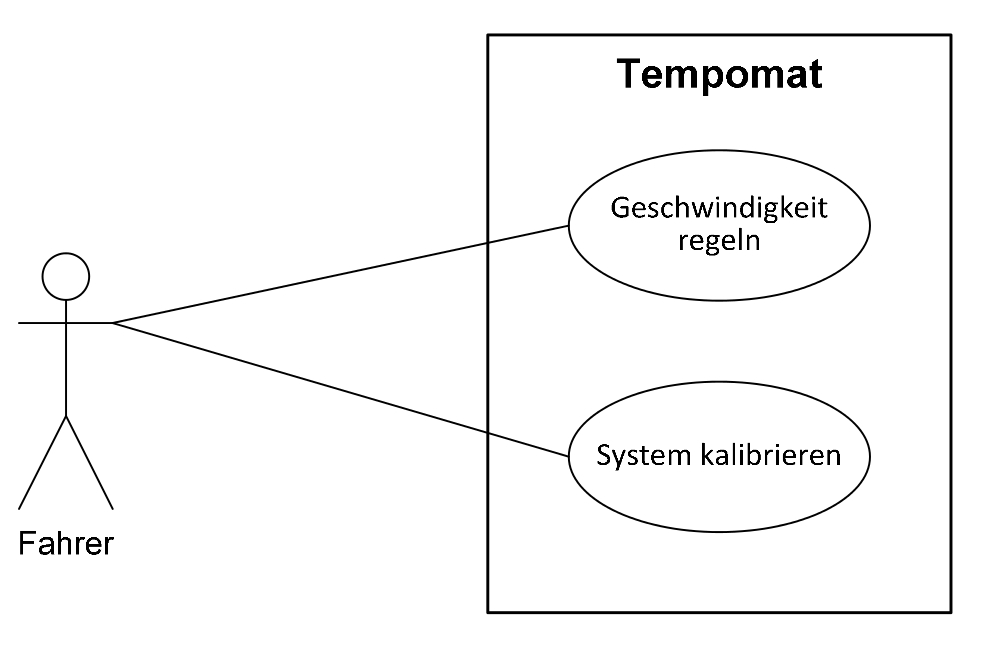
\includegraphics[height=8cm, width = 10cm,]{images/Modellierung/Systemgrenze} 	
	\label{fig:Systemgrenze}}
\end{figure} 

Aktoren sind: Menschen, Sensoren, Ein- und Ausgabegeräte, Nachbarsysteme, Zeit.\\ \\

\textbf{Systemprozesse finden}\\
Die Aufteilung in Hardware und Software sollte erst nach der Analyse der grundlegenden Anforderungen erfolgen.
Dieser Schritt ist in der Analysephase. Wenn hier von Prozessen die Rede ist, bedeutet das nicht unbedingt ein
Betriebssystem Prozess ist.








\subsection{Systemprozesse Detaillieren}

\subsection{Aktivitätsdiagramme}

\subsection{Zustandsbasierte Systeme}